% Relevant evidence per retrieval step on holdout 3 (run a) and cumulative over the agent's searches.
\begin{figure}[htbp]
\centering
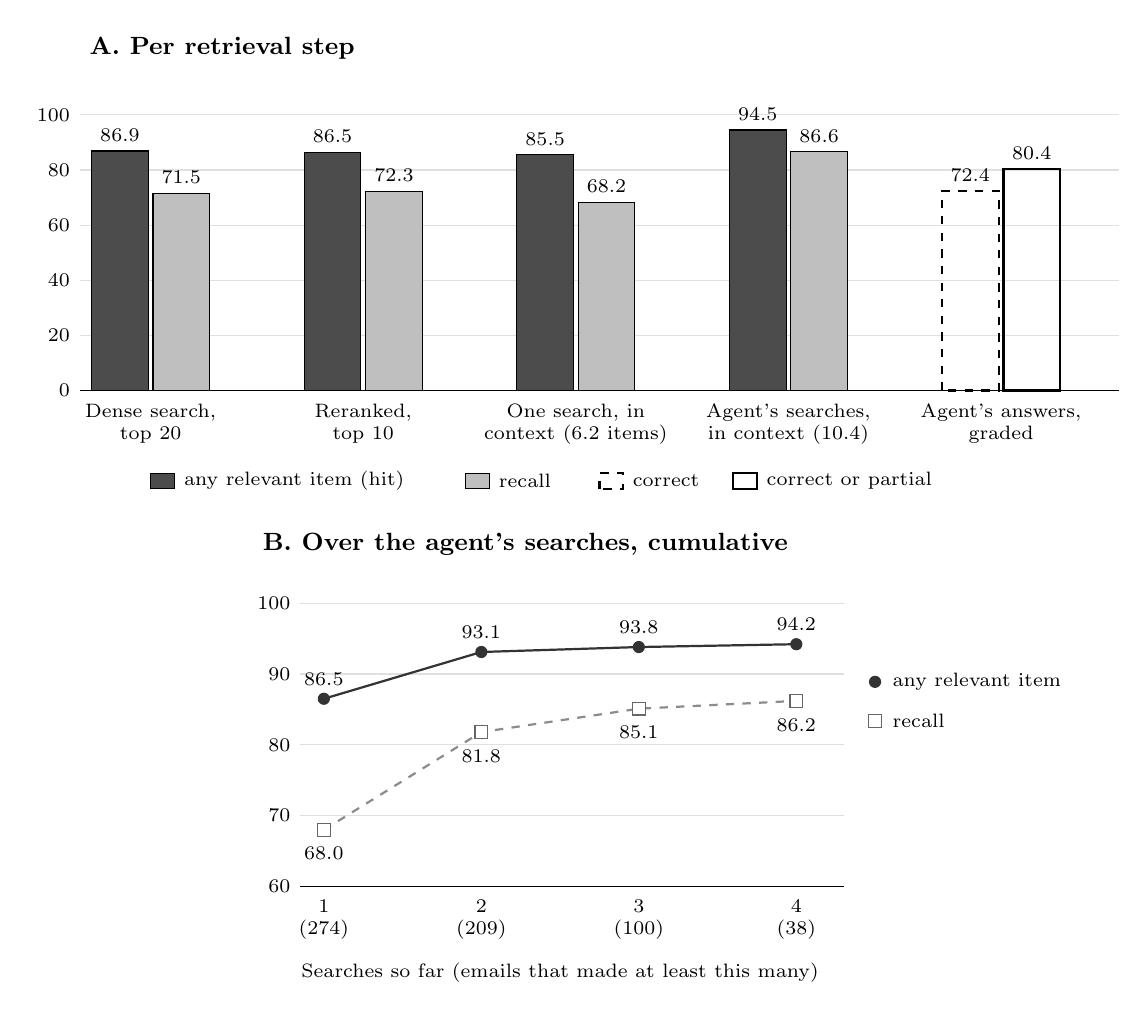
\begin{tikzpicture}[x=1cm,y=1cm,font=\small]
  % panel A: per step
  \node[anchor=west,font=\small\bfseries] at (-0.9,4.35) {A. Per retrieval step};
  \foreach \p in {0,20,40,60,80,100} {
    \draw[black!12] (-0.9,{\p*0.035}) -- (12.3,{\p*0.035});
    \node[left,font=\scriptsize] at (-0.9,{\p*0.035}) {\p};
  }
  \foreach \x/\h/\r/\lab in {0/86.9/71.5/{Dense search,\\top 20},
                             2.7/86.5/72.3/{Reranked,\\top 10},
                             5.4/85.5/68.2/{One search, in\\context (6.2 items)},
                             8.1/94.5/86.6/{Agent's searches,\\in context (10.4)}} {
    \fill[black!70,draw=black] (\x-0.75,0) rectangle (\x-0.03,{\h*0.035});
    \fill[black!25,draw=black] (\x+0.03,0) rectangle (\x+0.75,{\r*0.035});
    \node[above,font=\scriptsize] at (\x-0.39,{\h*0.035}) {\h};
    \node[above,font=\scriptsize] at (\x+0.39,{\r*0.035}) {\r};
    \node[below,align=center,font=\scriptsize] at (\x,-0.05) {\lab};
  }
  \draw[thick,dashed] (10.8-0.75,0) rectangle (10.8-0.03,{72.4*0.035});
  \draw[thick] (10.8+0.03,0) rectangle (10.8+0.75,{80.4*0.035});
  \node[above,font=\scriptsize] at (10.8-0.39,{72.4*0.035}) {72.4};
  \node[above,font=\scriptsize] at (10.8+0.39,{80.4*0.035}) {80.4};
  \node[below,align=center,font=\scriptsize] at (10.8,-0.05) {Agent's answers,\\graded};
  \draw (-0.9,0) -- (12.3,0);
  % legend
  \fill[black!70,draw=black] (0,-1.25) rectangle (0.3,-1.05); \node[right,font=\scriptsize] at (0.3,-1.15) {any relevant item (hit)};
  \fill[black!25,draw=black] (4.0,-1.25) rectangle (4.3,-1.05); \node[right,font=\scriptsize] at (4.3,-1.15) {recall};
  \draw[thick,dashed] (5.7,-1.25) rectangle (6.0,-1.05); \node[right,font=\scriptsize] at (6.0,-1.15) {correct};
  \draw[thick] (7.4,-1.25) rectangle (7.7,-1.05); \node[right,font=\scriptsize] at (7.7,-1.15) {correct or partial};

  % panel B: cumulative over agent searches
  \begin{scope}[yshift=-6.3cm,xshift=2.2cm]
    \node[anchor=west,font=\small\bfseries] at (-0.9,4.35) {B. Over the agent's searches, cumulative};
    \foreach \p in {60,70,80,90,100} {
      \draw[black!12] (-0.3,{(\p-60)*0.09}) -- (6.6,{(\p-60)*0.09});
      \node[left,font=\scriptsize] at (-0.3,{(\p-60)*0.09}) {\p};
    }
    \draw (-0.3,0) -- (6.6,0);
    \draw[black!80,thick] (0,{(86.5-60)*0.09}) -- (2,{(93.1-60)*0.09}) -- (4,{(93.8-60)*0.09}) -- (6,{(94.2-60)*0.09});
    \draw[black!45,thick,dashed] (0,{(68.0-60)*0.09}) -- (2,{(81.8-60)*0.09}) -- (4,{(85.1-60)*0.09}) -- (6,{(86.2-60)*0.09});
    \foreach \x/\h/\r/\n/\k in {0/86.5/68.0/274/1, 2/93.1/81.8/209/2, 4/93.8/85.1/100/3, 6/94.2/86.2/38/4} {
      \fill[black!80] (\x,{(\h-60)*0.09}) circle (2.2pt);
      \node[above,font=\scriptsize] at (\x,{(\h-60)*0.09+0.05}) {\h};
      \fill[white,draw=black!60] (\x-0.08,{(\r-60)*0.09-0.08}) rectangle (\x+0.08,{(\r-60)*0.09+0.08});
      \node[below,font=\scriptsize] at (\x,{(\r-60)*0.09-0.1}) {\r};
      \node[below,align=center,font=\scriptsize] at (\x,-0.05) {\k\\(\n)};
    }
    \node[below,font=\scriptsize] at (3,-0.85) {Searches so far (emails that made at least this many)};
    \fill[black!80] (7.0,2.6) circle (2.2pt); \node[right,font=\scriptsize] at (7.1,2.6) {any relevant item};
    \fill[white,draw=black!60] (6.92,2.02) rectangle (7.08,2.18); \node[right,font=\scriptsize] at (7.1,2.1) {recall};
  \end{scope}
\end{tikzpicture}
\caption[Relevant evidence per retrieval step and over the agent's searches]{Relevant evidence per retrieval step and over the agent's searches, on the 275 holdout-3 emails with a relevant item (AI relevance labels). Panel A follows one search through the pipeline: the dense candidates, the reranked top 10, and what passes the floor and the limit into the context. It then shows the context after all of the agent's searches, and the share of the agent's answers (run $a$) graded correct, or correct or partial. Panel B adds the agent's searches one at a time from its recorded tool outputs. An email that stopped earlier keeps its last value.}
\label{fig:recall-steps}
\end{figure}
